%-------------------------------------------------------------------------------
%                                PREAMBLE
%-------------------------------------------------------------------------------
\documentclass[usenames,dvipsnames,svgnames,10pt,aspectratio=169]{beamer}
%
\usefonttheme{professionalfonts}
% This theme uses TIKZ: compile twice with PDFLaTeX or LuaLaTeX.
%
%  Options:
%  - [clean]:    clean slides, i.e. logos and footbar are removed
%  - [kth]:      footbar style inspierd to the official KTH template
%  - [nicewave]: a different style of wave is used (not approved by FLOW)
%
\usetheme[clean]{flow}

\usepackage{tikz}

\usetikzlibrary{arrows}
\usetikzlibrary{shapes.geometric, math, positioning, calc, patterns, angles, quotes}
\usetikzlibrary{patterns.meta,decorations.pathmorphing}

\newcommand{\semaphore}[3]{% #1: color of circle,
                           % #2: color of semicircle
                           % #3: angle of semicircle 
  \tikz[node distance=0mm,baseline]
       {
         \node (s1) [circle, fill=#1, minimum size=6mm] {};
         \node      [semicircle, fill=#2, 
           inner sep=0pt, outer sep=0pt, minimum size=3mm,
           anchor=south,
           at={(s1.center)}, rotate=#3] {};
       }
}

\usepackage[]{circuitikz}

\usepackage{pgfplots}
\usepgfplotslibrary{polar}

\usepackage{hyperref,graphicx,lmodern}
\usepackage[utf8]{inputenc}
\usepackage{media9}
\usepackage{xcolor}
\usepackage{stmaryrd}
\usepackage{nicefrac}
\usepackage{multimedia}
\usepackage{multicol}
\usepackage{upgreek}
\usepackage[]{bm}
\usepackage[]{url}
\usepackage[]{animate}
\usepackage{amsmath}

\usepackage[most]{tcolorbox}

\newcommand*{\TakeFourierOrnament}[1]{{%
    \fontencoding{U}\fontfamily{futs}\selectfont\char#1}}
\newcommand*{\danger}{\TakeFourierOrnament{66}}

\graphicspath{{imgs/}}
\setbeamertemplate{blocks}[rounded][shadow=true]

\DeclareMathOperator*{\maximize}{maximize~}

%-------------------------------------------------------------------------------
%                                TITLE PAGE
%-------------------------------------------------------------------------------
\title[Nonlinear physics] % Short title used in footline
{
	Weakly nonlinear \\
  oscillators
}

\author[J.-Ch.~Loiseau] % Presenting author in short form used in footline
{
	\underline{Jean-Christophe Loiseau}
}
% - Give the names in the same order as the appear in the paper.
% - Underline the presenting author.

\institute[unused]
{
	\url{jean-christophe.loiseau@ensam.eu} \\
	Laboratoire DynFluid \\
	Arts et M\'etiers, France.
}
% Keep it simple, no one is interested in your street address.

% University logo(s)
\logot{
\includegraphics[width=.128\paperwidth]{DynFluid_logo}}  % Top logo
\logob{
\includegraphics[width=0.128\paperwidth]{ENSAM_logo}} % Bottom logo
% \logoc[{\includegraphics[width=.128\paperwidth]{limsi}}]{\includegraphics[width=.128\paperwidth]{limsi}} % Corner logo
%
% Cover image: \cvrimg{x position}{y position}{cover image}
\cvrimg{.77}{.8}{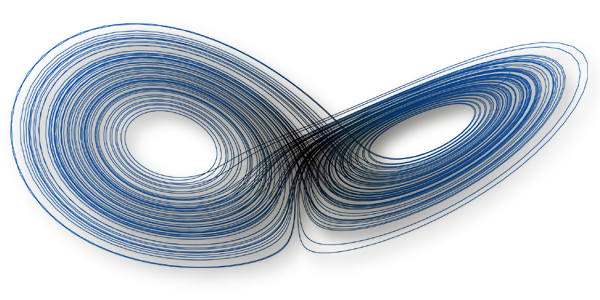
\includegraphics[width=.4\paperwidth]{cover.png}}

\date[unused]{Physique non-lin\'eaire -- 2019-2020}

\begin{document}

\titleframe	% Print the title as the first slide

%-------------------------------------------------------------------------------
%                           PRESENTATION SLIDES
%-------------------------------------------------------------------------------

\begin{frame}[t, c]{Weakly nonlinear oscillators}{Perturbation of the harmonic oscillator}

  \[
  \tcboxmath[colframe=beamer@kthblue, colback=white]{ \ddot{x} + x + \epsilon h(x, \dot{x}) = 0 }
  \]
  
  \bigskip
  
  For $0 \leq \epsilon \ll 1$ and $h(x, \dot{x})$ an arbitrary smooth function, this is known as a \alert{\textbf{weakly nonlinear oscillator}}.
  Because $\epsilon$ is small, they represent small perturbations of the \alert{\textbf{harmonic oscillator}}.

\end{frame}




\begin{frame}[t, c]{Weakly nonlinear oscillators}{Examples : the simple pendulum}
  \begin{minipage}{.68\textwidth}
    \[
    \tcboxmath[colframe=beamer@kthblue, colback=white]{ \textbf{Simple pendulum :} \quad \ddot{\theta} + \sin(\theta) }
    \]

    \bigskip

    For small angles, $\sin$ can be replaced by its Taylor series.
    The equation of motion becomes
    %
    \[
    \ddot{\theta} + \theta - \dfrac{\theta^3}{6} = 0.
    \]
    %
    The \alert{\textbf{periodic dynamics}} can be analyzed by means of the \alert{\textbf{Poincaré-Lindsted method}}.
  \end{minipage}%
  \hfill
  \begin{minipage}{.28\textwidth}
    \centering
    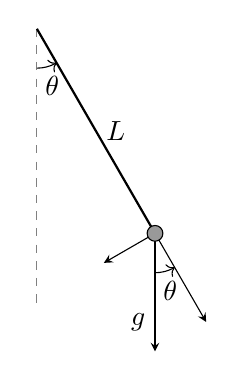
\begin{tikzpicture}
      % save length of g-vector and theta to macros
      \pgfmathsetmacro{\Gvec}{1.5}
      \pgfmathsetmacro{\myAngle}{30}
      % calculate lengths of vector components
      \pgfmathsetmacro{\Gcos}{\Gvec*cos(\myAngle)}
      \pgfmathsetmacro{\Gsin}{\Gvec*sin(\myAngle)}
      
      \coordinate (centro) at (0,0);
      \draw[dashed,gray,-] (centro) -- ++ (0,-3.5) node (mary) [black,below]{$ $};
      \draw[thick] (centro) -- ++(270+\myAngle:3) coordinate (bob) node[midway, right] {$L$};
      \pic [draw, ->, "$\theta$", angle eccentricity=1.5] {angle = mary--centro--bob};
      %\draw [blue,-stealth] (bob) -- ($(bob)!\Gcos cm!(centro)$);
      \draw [-stealth] (bob) -- ($(bob)!-\Gcos cm!(centro)$)
      coordinate (gcos)
      node[midway,above right] {};
      \draw [-stealth] (bob) -- ($(bob)!\Gsin cm!90:(centro)$)
      coordinate (gsin)
      node[midway,above left] {};
      \draw [-stealth] (bob) -- ++(0,-\Gvec)
      coordinate (g)
      node[near end,left] {$g$};
      \pic [draw, ->, "$\theta$", angle eccentricity=1.5] {angle = g--bob--gcos};
      \filldraw [fill=black!40,draw=black] (bob) circle[radius=0.1];
    \end{tikzpicture}
  \end{minipage}

  \vspace{1cm}
\end{frame}





\begin{frame}[t, c]{Weakly nonlinear oscillators}{Examples : the simple pendulum}
  \centering
  \begin{tikzpicture}[>=stealth]
    \draw[->] (-1.25*pi, 0) -- (1.25*pi, 0) node[below] {$\theta$};
    \draw[->] (0, -pi) -- (0, pi) node[left] {$\dot{\theta}$};
    
    \draw[gray, smooth, thick] plot file{pendulum_traj_1.txt};
    \draw[gray, smooth, thick] plot file{pendulum_traj_2.txt};
    \draw[gray, smooth, thick] plot file{pendulum_traj_3.txt};
    \draw[gray, smooth, thick] plot file{pendulum_traj_4.txt};
    \draw[gray, smooth, thick] plot file{pendulum_traj_5.txt};
    
    \draw[blue, dashed, smooth, thick] plot file{approx_traj_1.txt};
    \draw[blue, dashed, smooth, thick] plot file{approx_traj_2.txt};
    \draw[blue, dashed, smooth, thick] plot file{approx_traj_3.txt};
    \draw[blue, dashed, smooth, thick] plot file{approx_traj_4.txt};
    
    \node[circle, fill=black, draw=black, inner sep=0pt, minimum size=4pt] at (0, 0) {};
    \node[circle, fill=white, draw=black, inner sep=0pt, minimum size=4pt] at (-pi, 0) {};
    \node[circle, fill=white, draw=black, inner sep=0pt, minimum size=4pt] at (pi, 0) {};
    
    \draw[gray, thick] (pi/4, pi-0.5) -- (pi/4+1, pi-0.5) node[right] {True solution};
    \draw[dashed, blue, thick] (-pi/4, pi-0.5) -- (-pi/4-1, pi-0.5) node[left] {$\mathcal{O}(\epsilon)$};
    \end{tikzpicture}
\end{frame}



\begin{frame}[t, c]{Weakly nonlinear oscillators}{Examples : the van der Pol oscillator}
  \begin{minipage}{.68\textwidth}
    \[
    \tcboxmath[colframe=beamer@kthblue, colback=white]{\textbf{van der Pol osc.\ :} \quad \ddot{x} + x + \epsilon \left( x^2 - 1 \right) \dot{x} = 0}
    \]

    \bigskip

    It is a canonical example of nonlinear oscillators proposed in 1927 by the Dutch electrical engineer Balthasar van der Pol.
  \end{minipage}%
  \hfill
  \begin{minipage}{.28\textwidth}
    \centering
    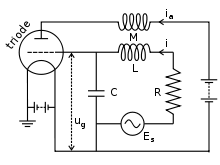
\includegraphics[width=\textwidth]{van_der_pol}
  \end{minipage}
\end{frame}

\begin{frame}[t, c]{Weakly nonlinear oscillators}{From the fixed point to the limit cycle}
  \begin{minipage}{.68\textwidth}

    Periodic limit cycle can be approximated by means of the Poincaré-Lindstedt method, but what about the \alert{\textbf{transient behaviour}}?

  \end{minipage}%
  \hfill
  \begin{minipage}{.28\textwidth}
    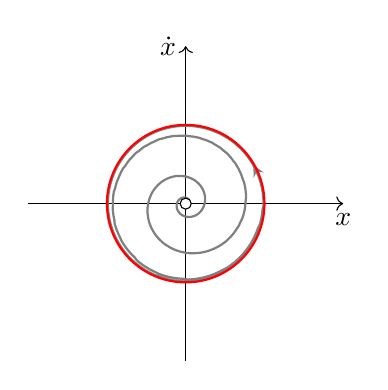
\begin{tikzpicture}
      \draw[->] (-2, 0) -- (2, 0) node[below] {$x$};
      \draw[->] (0, -2) -- (0, 2) node[left] {$\dot{x}$};

      \draw[->, >=stealth, gray, domain=0:50, variable=\t, samples=1024, thick] plot ({2*sqrt(0.25*0.001 / (0.001 + exp(-0.5*\t)*(0.25-0.001))) * cos((\t+pi/4) r)}, {2*sqrt(0.25*0.001 / (0.001 + exp(-0.5*\t)*(0.25-0.001))) * sin((\t+pi/4) r)});

      \node[circle, fill=white, draw=black, inner sep=0pt, minimum size=4pt] (a) at (0, 0) {};

      \draw[red, thick] (0, 0) circle (1);
    \end{tikzpicture}
  \end{minipage}

  \vspace{1cm}
\end{frame}

\begin{frame}[t, c]{Weakly nonlinear oscillators}{The failure of regular perturbation theory}
  \begin{minipage}{.68\textwidth}

    \[
    \tcboxmath[colframe=beamer@kthblue, colback=white]{\textbf{Weakly nonlin.\ osc.\ :} \quad \ddot{x} + x + \epsilon h(x, \dot{x}) = 0 }
    \]

    \bigskip

    It is natural to seek an approximate solution in the form of a power series in $\epsilon$, i.e.
    %
    \[
    x(t, \epsilon) = x_0(t) + \epsilon x_1(t) + \epsilon^2 x_2(t) + \cdots
    \]
    %
    This is known as \alert{\textbf{regular perturbation theory}} but it is doomed to fail...
  \end{minipage}%
  \hfill
  \begin{minipage}{.28\textwidth}
    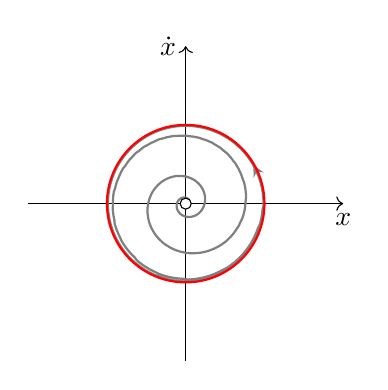
\begin{tikzpicture}
      \draw[->] (-2, 0) -- (2, 0) node[below] {$x$};
      \draw[->] (0, -2) -- (0, 2) node[left] {$\dot{x}$};

      \draw[->, >=stealth, gray, domain=0:50, variable=\t, samples=1024, thick] plot ({2*sqrt(0.25*0.001 / (0.001 + exp(-0.5*\t)*(0.25-0.001))) * cos((\t+pi/4) r)}, {2*sqrt(0.25*0.001 / (0.001 + exp(-0.5*\t)*(0.25-0.001))) * sin((\t+pi/4) r)});

      \node[circle, fill=white, draw=black, inner sep=0pt, minimum size=4pt] (a) at (0, 0) {};

      \draw[red, thick] (0, 0) circle (1);
    \end{tikzpicture}
  \end{minipage}

\end{frame}





\begin{frame}[t, c]{Weakly nonlinear oscillators}{The failure of regular perturbation theory}
  \begin{minipage}{.68\textwidth}
    Consider $h(x, \dot{x}) = 2\dot{x}$.
    The system considered is thus the \alert{\textbf{weakly damped linear oscillator}}
    %
    \[
    \ddot{x} + 2\epsilon \dot{x} + x = 0.
    \]
    %
    For $x(0) = 0$ and $\dot{x}(0) = 1$, its solution is
    %
    \[
    x(t, \epsilon) = \dfrac{1}{\sqrt{1 - \epsilon^2}} \sin\left(\sqrt{1 - \epsilon^2} t \right) e^{-\epsilon t}.
    \]
    %
    Let us now approximate this solution with regular perturbation theory.
  \end{minipage}%
  \hfill
  \begin{minipage}{.28\textwidth}
  \centering
  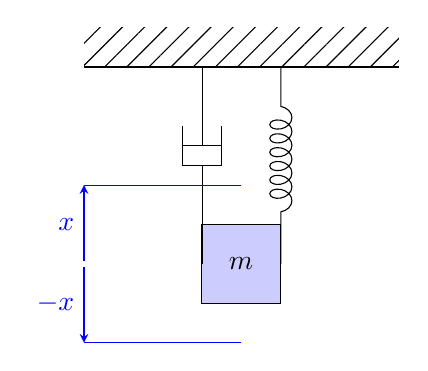
\begin{tikzpicture}[>=stealth]
      \path[pattern={Lines[angle=45,distance={8pt/sqrt(2)}]}] (-2, 5) edge ++(4,0) rectangle ++ (4, 0.5);

      \draw[decorate,decoration={coil, segment length=5pt, aspect=0.7, amplitude=4pt,
          pre=lineto, pre length=5mm, post=lineto, post length=5mm}] (0.5, 5) -- (0.5, 2.5)
      node[left, draw, minimum size=1cm, fill=blue!20] (m) {$m$};

      \draw[] (-0.5, 5) -- (-0.5, 4) {};
      \draw[] (-0.25, 4) -- (-0.75, 4) {};

      \draw[] (-0.5, 3.75) -- (-0.5, 2.5) {};
      \draw[] (-0.25, 3.75) -- (-0.75, 3.75) {};

      \draw[] (-0.25, 3.75) -- (-0.25, 4.25) {};
      \draw[] (-0.75, 3.75) -- (-0.75, 4.25) {};

      \draw[blue] (m.center-|0, 0) ++ (0, 1) -- ++ (-2, 0)
      edge[<-,edge label'=$x$,shorten >=1pt] (m.center-|-2, 0)
      (m.center-|0, 0) ++ (0, -1) -- ++ (-2, 0) 
      edge[<-,edge label=$-x$,shorten >=1pt] (m.center-|-2, 0);
      %(m.east) edge[dashed] (m.east-|2, 0) 
      %(m.east-|2, 0) node[right] {Equilibrium};
  \end{tikzpicture}
  \end{minipage}
\end{frame}




\begin{frame}[t, c]{Weakly nonlinear oscillators}{The failure of regular perturbation theory}
  Introducing our power series expansion into the equation leads to
  %
  \[
  \dfrac{d^2}{dt^2}\left( x_0 + \epsilon x_1 + \cdots \right) + 2\epsilon \dfrac{d}{dt} \left( x_0 + \epsilon x_1 + \cdots \right) + \left( x_0 + \epsilon x_1 + \cdots \right) = 0.
  \]
  %
  Grouping terms by powers of $\epsilon$, we get
  %
  \[
  \tcboxmath[colframe=beamer@kthblue, colback=white]{
    \begin{aligned}
      \mathcal{O}(1) : \quad & \ddot{x}_0 + x_0 = 0 \\
      \mathcal{O}(\epsilon) : \quad & \ddot{x}_1 + 2\dot{x}_0 + x_1 = 0.
    \end{aligned}
  }
  \]
  %
  with initial conditions $x_0(0) = x_1(0) = 0$ along with $\dot{x}_0 = 1$ and $\dot{x}_1(0) = 0$.
\end{frame}




\begin{frame}[t, c]{Weakly nonlinear oscillators}{The failure of regular perturbation theory}
  \[
  \tcboxmath[colframe=beamer@kthblue, colback=white]{
    \begin{aligned}
      \mathcal{O}(1) : \quad & \ddot{x}_0 + x_0 = 0 \\
      & x_0(0) = 0, \quad \dot{x}_0(0) = 1.
    \end{aligned}
  }
  \]
  
  \bigskip
  
  The zeroth-order solution is simply given by
  %
  \[
  x_0(t) = \sin(t).
  \]
  %
  In the absence of friction, the dynamics are simply periodic in time.
\end{frame}




\begin{frame}[t, c]{Weakly nonlinear oscillators}{The failure of regular perturbation theory}
  \[
  \tcboxmath[colframe=beamer@kthblue, colback=white]{
    \begin{aligned}
      \mathcal{O}(\epsilon) : \quad & \ddot{x}_1 + x_1 = -2\cos(t) \\
      & x_1(0) = 0, \quad \dot{x}_1(0) = 0.
    \end{aligned}
  }
  \]
  
  \bigskip
  
  {\large \danger} The right-hand side is a \alert{\textbf{resonant}} forcing !
  The first-order correction is given by
  %
  \[
  x_1(t) = -t \sin(t)
  \]
  %
  which is a \alert{\textbf{secular}} term, i.e. it grows without bound as $t \to \infty$.
  
\end{frame}




\begin{frame}[t, c]{Weakly nonlinear oscillators}{The failure of regular perturbation theory}

  \centering

  \[
  \tcboxmath[colframe=beamer@kthblue, colback=white]{
    \textbf{Perturbation theory :} \quad x(t, \epsilon) = \sin(t) - \epsilon t \sin(t) + \mathcal{O}(\epsilon^2)
  }
  \]

  \bigskip

  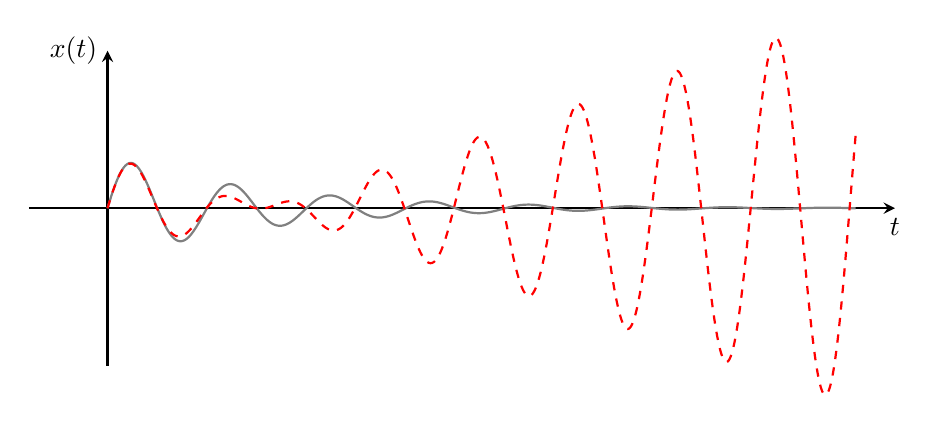
\begin{tikzpicture}[>=stealth]
    \draw[->, thick] (-1, 0) -- (10, 0) node[below] {$t$};
    \draw[->, thick] (0, -2) -- (0, 2) node[left] {$x(t)$};

    \draw[gray, domain=0:9.5, thick, smooth, samples=1024] plot (\x, {(2/3)*(sin(sqrt(1-0.1^2)*5*\x r)*exp(-0.1*5*\x)/sqrt(1-0.1^2))});

    \draw[dashed, red, domain=0:9.5, thick, smooth, samples=1024] plot (\x, {(2/3)*(sin(5*\x r) - 0.1 * 5*\x * sin(5*\x r))});
  \end{tikzpicture}

  \vspace{1cm}
\end{frame}




\begin{frame}[t, c]{Weakly nonlinear oscilators}{The failure of regular peturbation theory}
  \centering

  \tcbox[colframe=beamer@kthblue, colback=white]{\textbf{Question 1 :} How is the regular perturbation theory solution related to the true solution ?}

  \bigskip

  \tcbox[colframe=beamer@kthblue, colback=white]{\textbf{Question 2 :} Why does regular perturbation theory fail to capture the correct behaviour ?}

\end{frame}




\begin{frame}[t, c]{Weakly nonlinear oscillators}{Regular perturbation theory vs.\ true solution}
  \[
  \tcboxmath[colframe=beamer@kthblue, colback=white]{\textbf{Analytic solution :} \quad x(t, \epsilon) = \dfrac{1}{\sqrt{1 - \epsilon^2}} \sin(\sqrt{1 - \epsilon^2} t) e^{-\epsilon t}}
  \]

  \bigskip

  \begin{overprint}
    \onslide<1>
    \centering \textbf{Taylor expansion}
    %
    \[
    \dfrac{1}{\sqrt{1 - \epsilon^2}} \simeq 1 + \dfrac{1}{2} \epsilon^2, \quad \sin(\sqrt{1 - \epsilon^2}t) \simeq \sin(t), \quad  e^{-\epsilon t} \simeq 1 - \epsilon t
    \]

    \onslide<2>

    Hence, the first-order Taylor expansion of the analytic solution is \( x(t, \epsilon) = \sin(t) - \epsilon t \sin(t) + \mathcal{O}(\epsilon^2) \).
    This is precisely the solution obtained using regular perturbation theory !

  \end{overprint}
\end{frame}




\begin{frame}[t, c]{Weakly nonlinear oscillators}{Why does it fail ?}
  \[
  \tcboxmath[colframe=beamer@kthblue, colback=white]{\textbf{Analytic solution :} \quad x(t, \epsilon) = \dfrac{1}{\sqrt{1 - \epsilon^2}} \sin(\sqrt{1 - \epsilon^2} t) e^{-\epsilon t}}
  \]

  \bigskip

  The true solution exhibits \alert{\textbf{two time scales}} : a \emph{fast time} $t \sim \mathcal{O}(1)$ for the sinusoidal oscillations and a \emph{slow time} $t \sim \nicefrac{1}{\epsilon}$ over which the amplitude decays.
  This slow time scale is completely misrepresented by the regular perturbation theory solution.

\end{frame}




\begin{frame}[t, c]{Weakly nonlinear oscillators}{Two time scales}
  \centering
  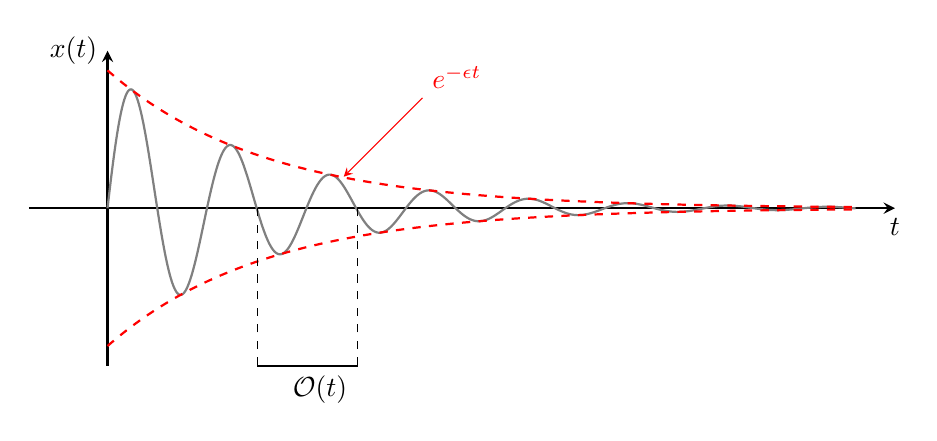
\begin{tikzpicture}[>=stealth]
    \draw[->, thick] (-1, 0) -- (10, 0) node[below] {$t$};
    \draw[->, thick] (0, -2) -- (0, 2) node[left] {$x(t)$};

    \draw[gray, domain=0:9.5, thick, smooth, samples=1024] plot (\x, {1.75*(sin(sqrt(1-0.1^2)*5*\x r)*exp(-0.1*5*\x)/sqrt(1-0.1^2))});

    \draw[red, domain=0:9.5, dashed, thick, smooth, samples=1024] plot (\x, {1.75*exp(-0.1*5*\x)});
    \draw[red, domain=0:9.5, dashed, thick, smooth, samples=1024] plot (\x, {-1.75*exp(-0.1*5*\x)});

    \draw[<-, red] (3, 0.4) -- (4, 1.4) node[above right] {$e^{-\epsilon t}$};

    \draw[-, black, thick] (1.9, -2) -- (3.175, -2) node[below left] {$\mathcal{O}(t)$};
    \draw[dashed, black] (1.9, -2) -- (1.9, 0) {};
    \draw[dashed, black] (3.175, -2) -- (3.175, 0) {};

  \end{tikzpicture}

\end{frame}






\begin{frame}[t, c]{Weakly nonlinear oscillators}{A two-time scales approach}
  \begin{minipage}{.68\textwidth}
    Multiple time scales are ubquituous in nonlinear oscillators.
    The phase tends to evolves at a much faster rate than the oscillation's amplitude.
    We thus need to explicitly take into account these two time scales when approximating the solution.
  \end{minipage}%
  \hfill
  \begin{minipage}{.28\textwidth}
    \centering
    \begin{tikzpicture}[>=stealth]
      \draw[->] (-2, 0) -- (2, 0) node[below] {$x$};
      \draw[->] (0, -2) -- (0, 2) node[left] {$\dot{x}$};
      
      \draw[gray, thick] plot file{van_der_pol_traj_bis.txt};
      
      \node[circle, fill=white, draw=black, inner sep=0pt, minimum size=4pt] at (0, 0) {};
    \end{tikzpicture}
  \end{minipage}
\end{frame}




\begin{frame}[t, c]{Weakly nonlinear oscillators}{Two-timing approach}
  \begin{center}
    \textbf{Idea :} Treat the two time scales as if they were independent.
  \end{center}

  \bigskip

  Let $\tau = t$ denote the $\mathcal{O}(1)$ time scale and $T = \epsilon t$ the slow one.
  Functions of the slow time $T$ will be regarded as \emph{constants} on the fast time scale $\tau$.
  Hard to justify rigorously but it works !
\end{frame}




\begin{frame}[t, c]{Weakly nonlinear oscillators}{Two-timing approach}
  As before, let us expand our solution as a power series in $\epsilon$
  %
  \[
  x(t, \epsilon) = x_0(\tau, T) + \epsilon x_1(\tau, T) + \mathcal{O}(\epsilon^2).
  \]

  \bigskip

  The time-derivatives in our governing equations are transformed using the chain rule.

  \bigskip

  \begin{minipage}{.32\textwidth}
    \[
      \dfrac{dx}{dt} = \dfrac{\partial x}{\partial \tau} + \epsilon \dfrac{\partial x}{\partial T}
    \]
  \end{minipage}%
  \hfill
  \begin{minipage}{.64\textwidth}
    \[
    \dfrac{d^2 x}{dt^2} = \dfrac{\partial^2 x}{\partial \tau^2} + 2\epsilon \dfrac{\partial^2 x}{\partial \tau \partial T} + \epsilon^2 \dfrac{\partial^2 x}{\partial T^2}
    \]
  \end{minipage}
\end{frame}




\begin{frame}[t, c]{Weakly nonlinear oscillators}{Two-timing approach}
  Introducing our power series expansion into the equation leads to
  %
  \[
  \dfrac{\partial^2 x_0}{\partial \tau^2} + \epsilon \left( \dfrac{\partial^2 x_1}{\partial \tau^2} + 2 \dfrac{\partial^2 x_0}{\partial \tau \partial T} \right) + 2\epsilon \dfrac{\partial x_0}{\partial \tau} + x_0 + \epsilon x_1 + \mathcal{O}(\epsilon^2) = 0.
  \]
  %
  Grouping by powers of $\epsilon$ yields
  %
  \[
  \tcboxmath[colframe=beamer@kthblue, colback=white]{
    \begin{aligned}
      \mathcal{O}(1) : \quad & \dfrac{\partial^2 x_0}{\partial \tau^2} + x_0 = 0 \\
      \mathcal{O}(\epsilon) : \quad & \dfrac{\partial^2 x_1}{\partial \tau^2} + 2 \dfrac{\partial^2 x_0}{\partial T \partial \tau} + 2 \dfrac{\partial x_0}{\partial \tau} + x_1 = 0 
    \end{aligned}
  }
  \]
  %
  along with appropriate initial conditions.
\end{frame}




\begin{frame}[t, c]{Weakly nonlinear oscilllators}{Two-timing approach}
  \[
  \tcboxmath[colframe=beamer@kthblue, colback=white]{
    \mathcal{O}(1) : \quad \dfrac{\partial^2 x_0}{\partial \tau^2} + x_0 = 0
  }
  \]

  \bigskip

  The general solution of the zeroth-order approximation is simply
  %
  \[
  x_0(\tau, T) = A(T) \sin(\tau) + B(T) \cos(\tau).
  \]
  %
  To determine the functions $A(T)$ and $B(T)$, one needs to go to the next order in $\epsilon$.

\end{frame}




\begin{frame}[t, c]{Weakly nonlinear oscillators}{Two-timing approach}
  \[
  \tcboxmath[colframe=beamer@kthblue, colback=white]{
    \mathcal{O}(\epsilon) : \quad \dfrac{\partial^2 x_1}{\partial \tau^2} + x_1 = -2 \left( \dfrac{dA}{dT} + A \right) \cos(\tau) + 2 \left( \dfrac{dB}{dT} + B \right) \sin(\tau)
  }
  \]

  \bigskip

  The right-hand side is a \alert{\textbf{resonant}} forcing that will lead to \alert{\textbf{secular growth}} unless $A$ and $B$ satisfy
  %
  \[
  \dfrac{dA}{dT} = - A, \quad \text{and} \quad \dfrac{dB}{dT} = -B
  \]
  %
  whose general solutions are given by $A(T) = A(0) e^{-T}$ and $B(T) = B(0) e^{-T}$.
\end{frame}




\begin{frame}[t, c]{Weakly nonlinear oscillators}{Two-timing approach}
  \centering

  \[
  \tcboxmath[colframe=beamer@kthblue, colback=white]{
    \textbf{Two-timing solution :} \quad x(t) = \sin(t) e^{-\epsilon t}
  }
  \]

  \bigskip

  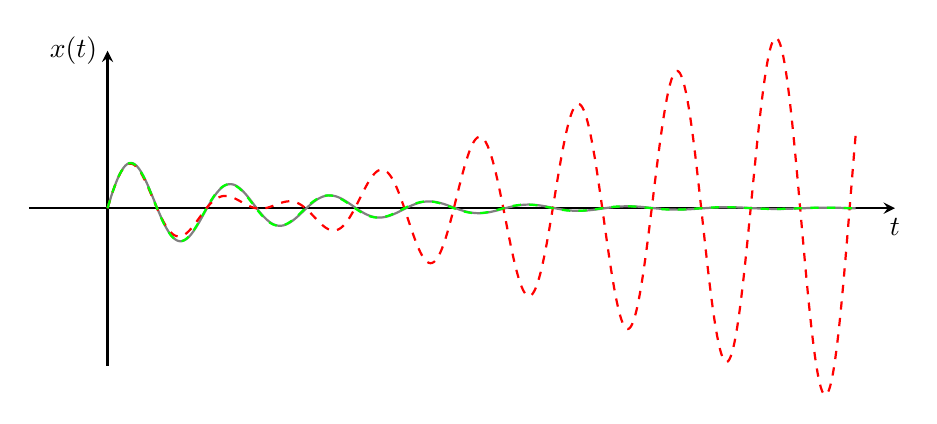
\begin{tikzpicture}[>=stealth]
    \draw[->, thick] (-1, 0) -- (10, 0) node[below] {$t$};
    \draw[->, thick] (0, -2) -- (0, 2) node[left] {$x(t)$};

    \draw[gray, domain=0:9.5, thick, smooth, samples=1024] plot (\x, {(2/3)*(sin(sqrt(1-0.1^2)*5*\x r)*exp(-0.1*5*\x)/sqrt(1-0.1^2))});

    \draw[dashed, red, domain=0:9.5, thick, smooth, samples=1024] plot (\x, {(2/3)*(sin(5*\x r) - 0.1 * 5*\x * sin(5*\x r))});

    \draw[dashed, green, domain=0:9.5, thick, smooth, samples=1024] plot (\x, {(2/3)*(sin(5*\x r)*exp(-0.1*5*\x))});
  \end{tikzpicture}

  \vspace{1cm}
\end{frame}

\end{document}
